\begin{comment}
\documentclass[10pt]{article}
\usepackage{fullpage, graphicx, url}
\setlength{\parskip}{1ex}
\setlength{\parindent}{0ex}
\title{GEN13}
\begin{document}


\begin{tabular}{ccc}
The Alternative Csound Reference Manual & & \\
Previous & &Next

\end{tabular}

%\hline 
\end{comment}
\section{GEN13}
GEN13�--� Stores a polynomial whose coefficients derive from the Chebyshev polynomials of the first kind. \subsection*{Description}


  Uses Chebyshev coefficients to generate stored polynomial functions which, under waveshaping, can be used to split a sinusoid into harmonic partials having a pre-definable spectrum. 
\subsection*{Syntax}


 \textbf{f}
 \# time size 13 xint xamp h0 h1 h2 ...
\subsection*{Initialization}


 \emph{size}
 -- number of points in the table. Must be a power of 2 or a power-of-2 plus 1 (see \emph{f statement}
). The normal value is power-of-2 plus 1. 


 \emph{xint}
 -- provides the left and right values [\emph{-xint, +xint}
] of the x interval over which the polynomial is to be drawn. These subroutines both call \emph{GEN03}
 to draw their functions; the p5 value here is therefor expanded to a negative-positive p5, p6 pair before \emph{GEN03}
 is actually called. The normal value is 1. 


 \emph{xamp }
 -- amplitude scaling factor of the sinusoid input that is expected to produce the following spectrum. 


 \emph{h0, h1, h2,}
 etc. -- relative strength of partials 0 (DC), 1 (fundamental), 2 ... that will result when a sinusoid of amplitude 


 xamp�*�int(size/2)/xint\\ 
 ������
 is waveshaped using this function table. These values thus describe a frequency spectrum associated with a particular factor \emph{xamp}
 of the input signal. 

 \emph{GEN13}
 is the function generator normally employed in standard waveshaping. It stores a polynomial whose coefficients derive from the Chebyshev polynomials of the first kind, so that a driving sinusoid of strength \emph{xamp}
 will exhibit the specified spectrum at output. Note that the evolution of this spectrum is generally not linear with varying \emph{xamp}
. However, it is bandlimited (the only partials to appear will be those specified at generation time); and the partials will tend to occur and to develop in ascending order (the lower partials dominating at low \emph{xamp}
, and the spectral richness increasing for higher values of \emph{xamp}
). A negative \emph{hn}
 value implies a 180 degree phase shift of that partial; the requested full-amplitude spectrum will not be affected by this shift, although the evolution of several of its component partials may be. The pattern +,+,-,-,+,+,... for \emph{h0,h1,h2..}
. will minimize the normalization problem for low \emph{xamp}
 values (see above), but does not necessarily provide the smoothest pattern of evolution. 
\subsection*{Examples}


  Here is a simple example of the GEN13 routine. It uses the files \emph{gen13.orc}
 and \emph{gen13.sco}
. It creates a function which, under waveshaping, will split a sinusoid into 3 odd-harmonic partials of relative strength 5:3:1. Here is its diagram: 


 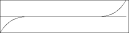
\includegraphics[scale=1]{gen13} 


 Diagram of the waveform generated by GEN13.


 \textbf{Example 1. A simple example of the GEN13 routine.}

\begin{lstlisting}
/* gen13.orc */
; Initialize the global variables.
sr = 44100
kr = 4410
ksmps = 10
nchnls = 1

; Instrument #1.
instr 1
  ; Create an index over the length of our entire note.
  kcps init 1/p3
  kndx phasor kcps

  ; Read Table #1 with our index.
  ifn = 1
  ixmode = 1
  kval table kndx, ifn, ixmode

  ; Generate a sine waveform, use our Table #1 value to
  ; vary its frequency by 100 Hz from its base frequency.
  ibasefreq = 440
  kfreq = kval * 100
  a1 oscil 20000, ibasefreq + kfreq, 2
  out a1
endin
/* gen13.orc */
        
\end{lstlisting}
\begin{lstlisting}
/* gen13.sco */
; Table #1: a polynomial function (using GEN13).
f 1 0 1025 13 1 1 0 5 0 3 0 1
; Table #2, a sine wave.
f 2 0 16384 10 1

; Play Instrument #1 for 2 seconds.
i 1 0 2
e
/* gen13.sco */
        
\end{lstlisting}
\subsection*{See Also}


 \emph{GEN03}
, \emph{GEN14}
, and \emph{GEN15}
. 
%\hline 


\begin{comment}
\begin{tabular}{lcr}
Previous &Home &Next \\
GEN12 &Up &GEN14

\end{tabular}


\end{document}
\end{comment}
